\section{Content}

Let's now move to the analysis of the content.
The page that we analyze in general is \url{https://siciliangoodness.shop/padovaviaroma/}. 
In general we can see that the back button works very well and from each page where we are, we can go back to the previous page.
An other important aspect is that we avoid the phenomenon of 'The lost in the navigation'. In fact, in the homepage, with the breadcrumbs, we always know where we are and the path that we follow. 

\begin{figure}[H]
	\centering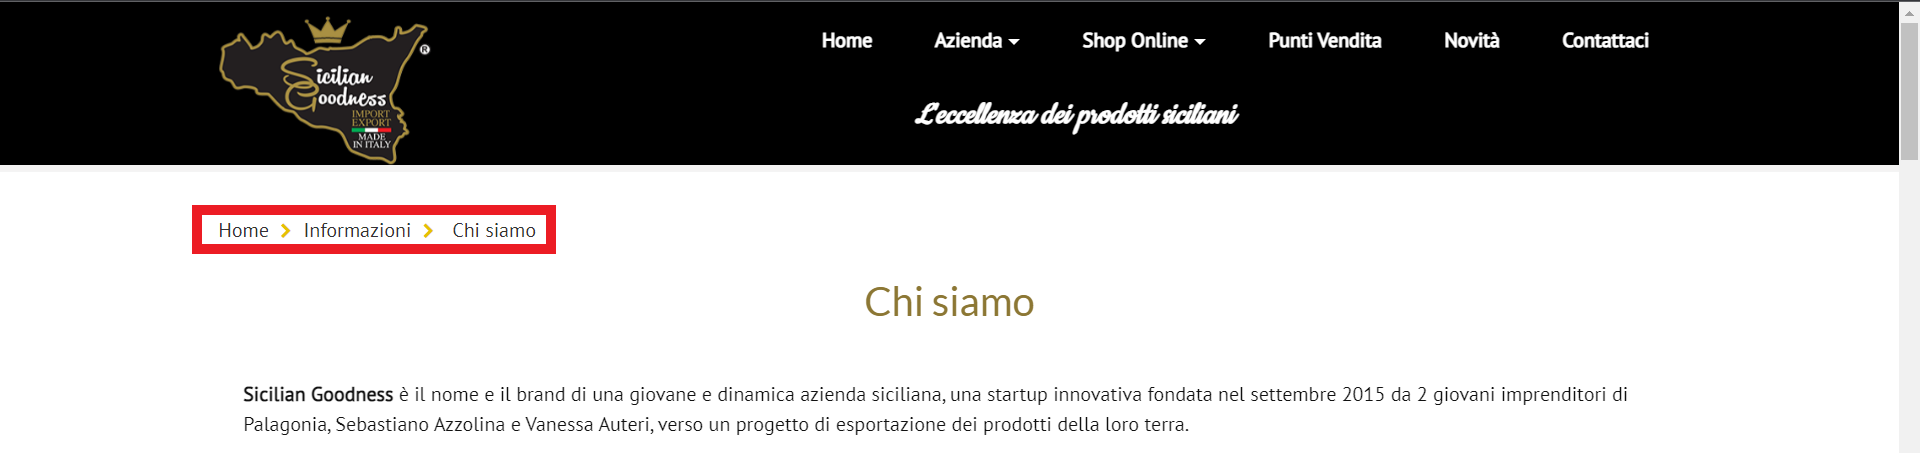
\includegraphics[width=12cm]{Img/bred2.png}
	\caption{Homepage Breadcrumb}
\end{figure}

The only pages that have some problems are 'SHOP VIGONZA' and SHOP PADOVA VIA ROMA'. Indeed in these pages it is difficult to come back to the homepage, because it seems to be a new page where you start your research. Indeed, we can see that no breadcrumbs are present and if we click on the logo we reload the same page. But if we click on a new page we start the navigation from this site.

\begin{figure}[H]
	\centering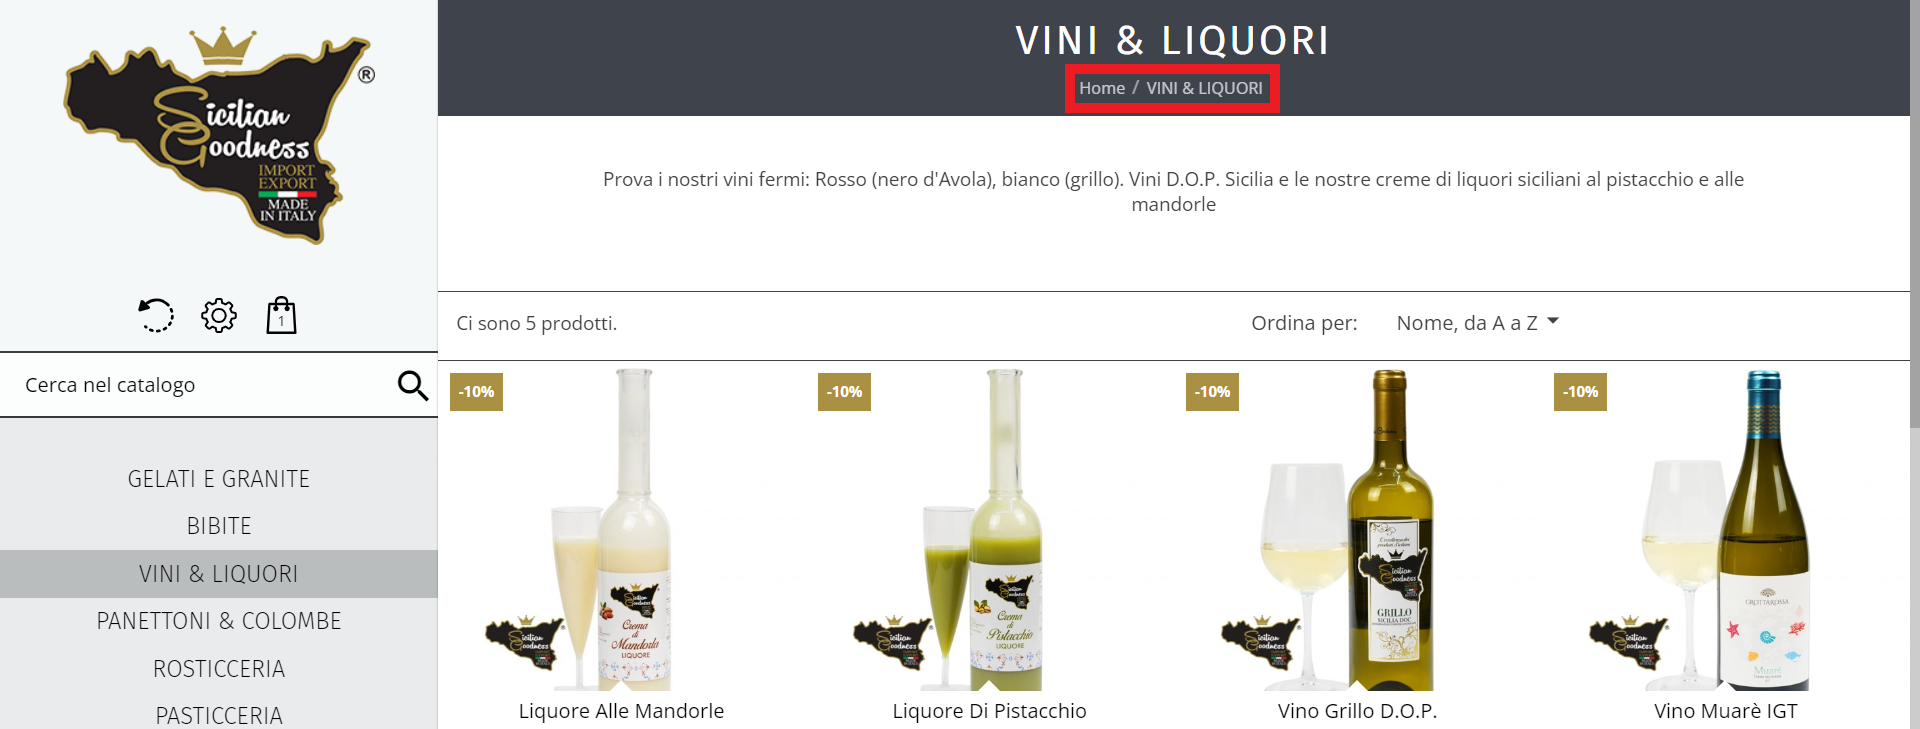
\includegraphics[width=12cm]{Img/bred1.png}
	\caption{Shop Breadcrumb}
\end{figure} 

In particular in this section we'll analyze the page to search the products and the 404 page will be briefly analyzed too. In conclusion we'll analyze the page of a single product (with the analysis of the Ws), as it is the most significant and most visited type of page.

\subsection{Shop}
The logo is well situated in the top-left corner of the website.
We don't deeply analyze the Ws but we can see in the image that the mandatory are present(Who: in the center, Where: in the center, What: in the left column).

\begin{figure}[H]
	\centering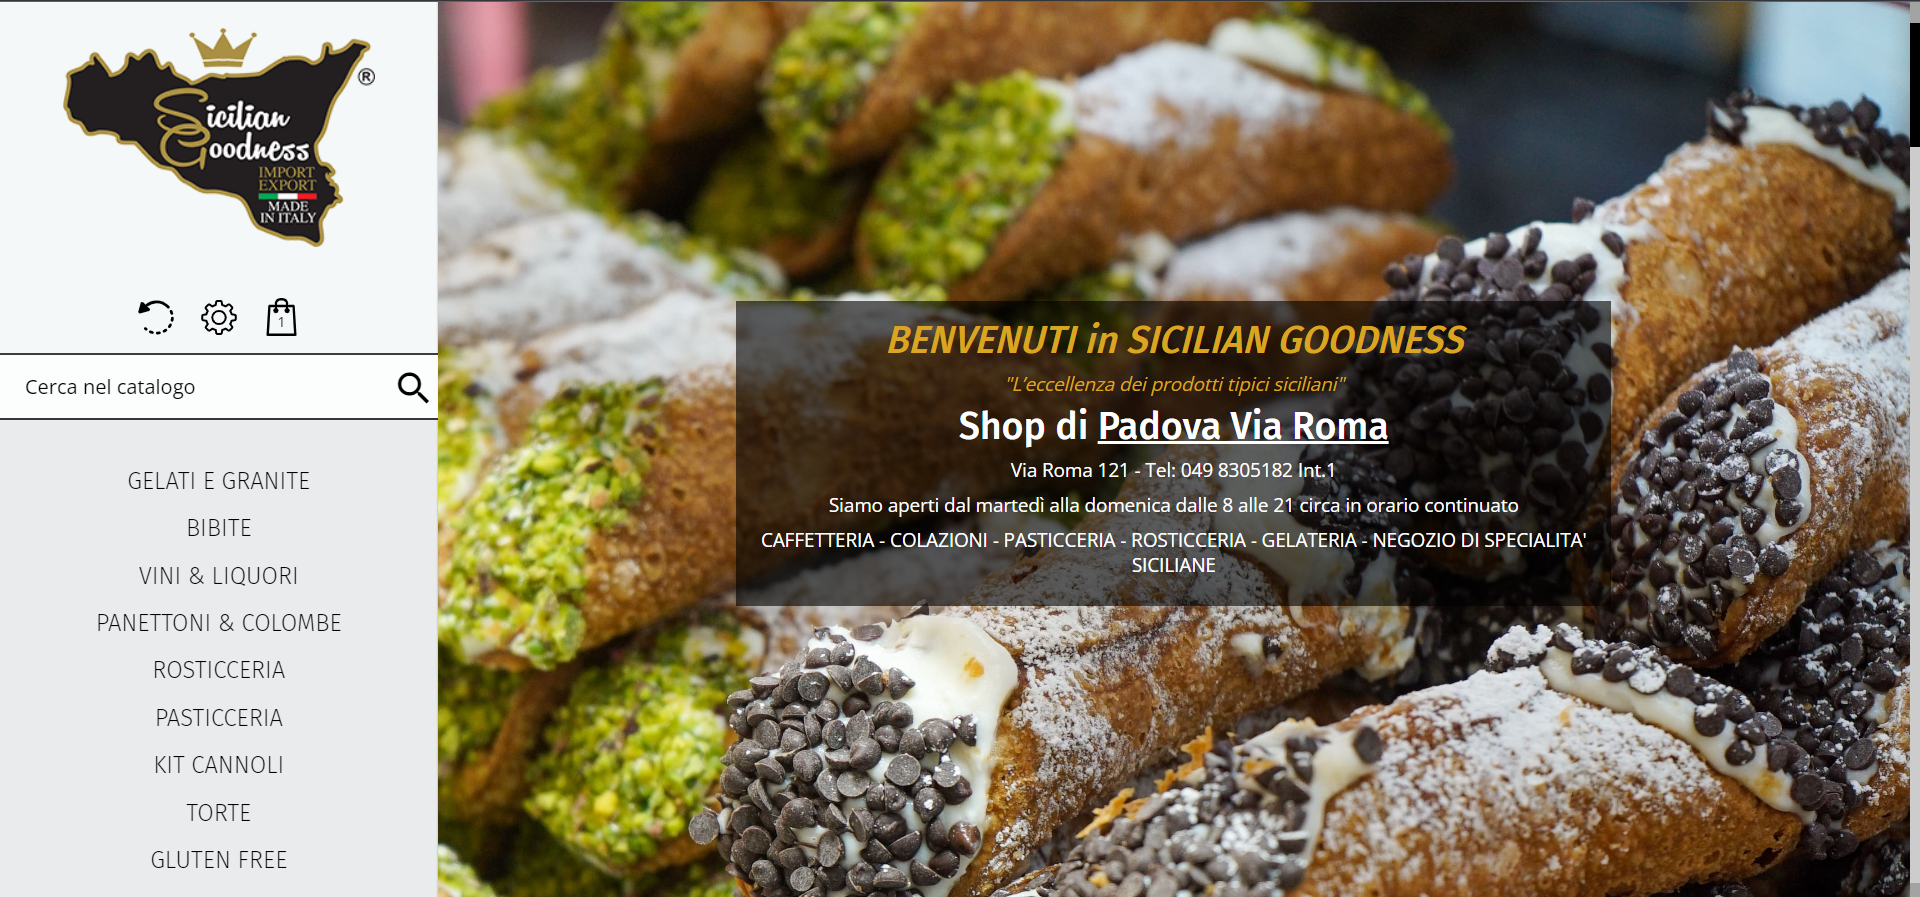
\includegraphics[width=12cm]{Img/Shop.png}
	\caption{Shop page}
\end{figure}

There is a lot of content in this page. In fact, for seeing all the information of the page we have to scroll more or less 7 times.
\newline
The menu is well structured vertically. In fact, the user can clearly search what he wants. 
Even the underlying menu is well structured. In fact, whit its design it avoid unwanted clicks.

\begin{figure}[H]
	\centering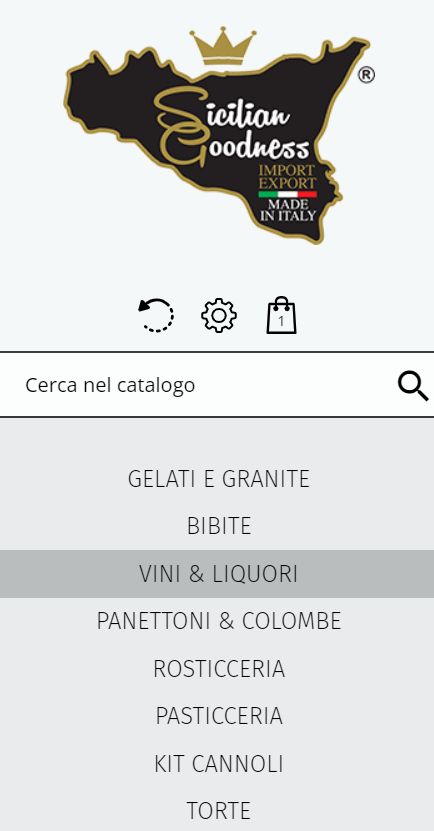
\includegraphics[height=12cm, width=7cm]{Img/menushop1.png}
	\caption{Menu Shop page 1}
\end{figure}

\begin{figure}[H]
	\centering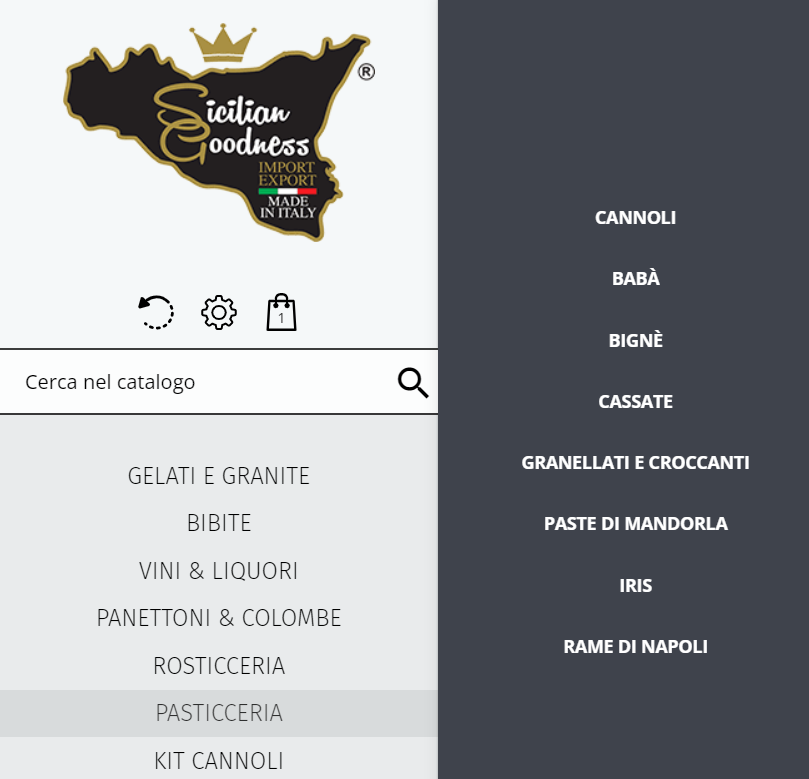
\includegraphics[height=12cm, width=12 cm]{Img/menushop2.png}
	\caption{Menu Shop page 2}
\end{figure}

To reload the page we can click on the logo or in the apposite icon under the logo.
On the right we find the registration button. 
This is an other important factor and the registration is not mandatory and is not forced in any way.

\subsection{Search}
ok
\subsubsection{Item}
Price 
media
...

\subsubsection{404}
ok

\begin{figure}[H]
	\centering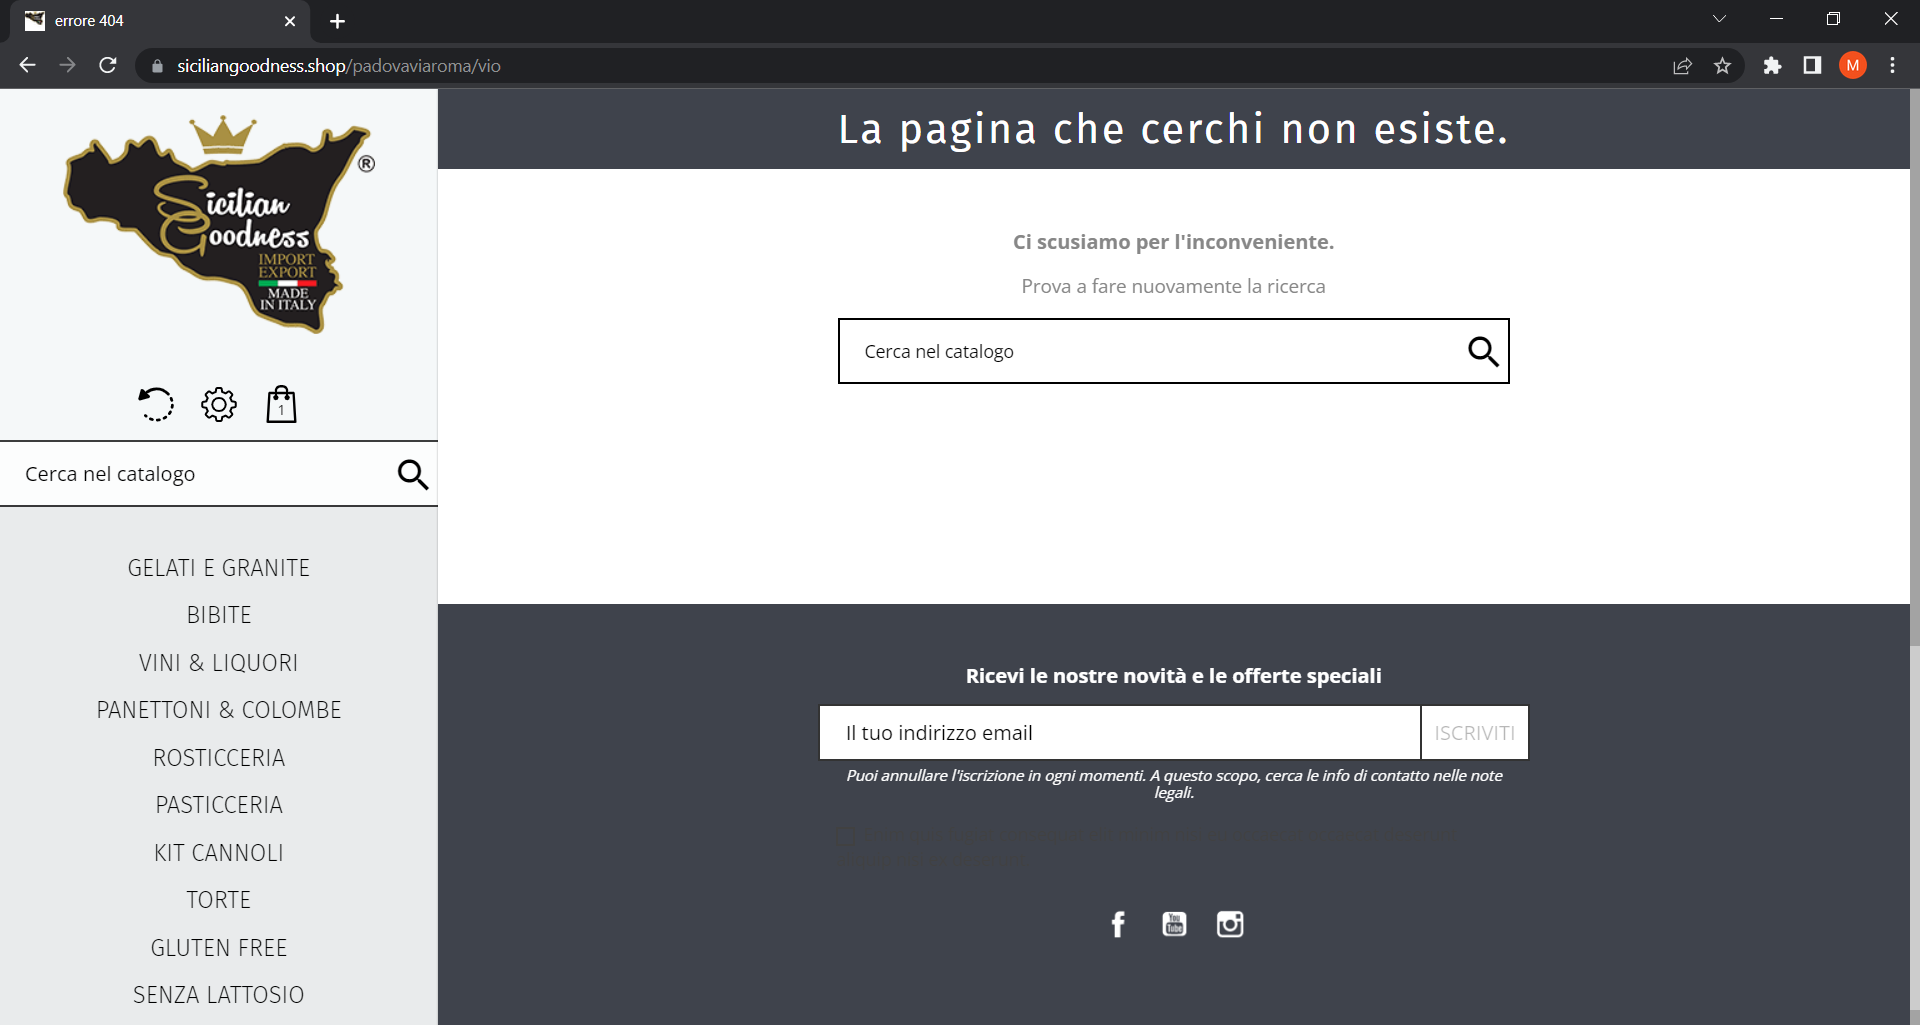
\includegraphics[width=12cm]{Img/404.png}
	\caption{404 page}
\end{figure}

\subsection{Product}
The page that we analyze is \url{https://siciliangoodness.shop/padovaviaroma/rosticceria/2-arancino-al-pistacchio.html}.

\subsubsection{The Six Ws}

\pagebreak